% !TeX root = tese.tex
%%% Exemplo de utilização da classe ITA
%%%
%%%   por        Fábio Fagundes Silveira   -  ffs [at] ita [dot] br
%%%              Benedito C. O. Maciel     -  bcmaciel [at] ita [dot] br
%%%              Giovani Volnei Meinertz   -  giovani [at] ita [dot] br
%%%    	         Hudson Alberto Bode       -  bode [at] ita [dot]br
%%%    	         P. I. Braga de Queiroz    -  pi [at] ita [dot] br
%%%    	         Jorge A. B. Gripp         -  gripp [at] ita [dot] br
%%%    	         Juliano Monte-Mor         -  jamontemor [at] yahoo [dot] com [dot] br
%%%    	         Tarcisio A. B. Gripp      -  tarcisio.gripp [at] gmail [dot] com
%%%
%%%   Versão para overleaf:
%%%   por        Alejandro A. Rios Cruz    - aarc.88@gmail.com
%%%              Saulo Gómez               - sagomezs@unal.edu.co
%%%              Ocimar Santos             - ocimar.acad@gmail.com
%%%
%%%   Template disponibilizado em:
%%%              Overleaf: https://pt.overleaf.com/latex/templates/thesis-template-aeronautics-institute-of-technology-ita/yhfrqqydpygk
%%%
%%%   Contribuia você também!
%%%              GitHub:   https://github.com/AlejandroRios/Template_Thesis_ITA
%%%
%%%  IMPORTANTE: O texto contido neste exemplo nao significa absolutamente nada.  :-)
%%%              O intuito aqui eh demonstrar os comandos criados na classe e suas
%%%              respectivas utilizacoes.
%%%
%%%  Tese.tex  2016-08-25
%%%  $HeadURL: http://www.apgita.org.br/apgita/teses-e-latex.php $
%%%
%%% ITALUS
%%% Instituto Tecnológico de Aeronáutica --- ITA, Sao Jose dos Campos, Brasil
%%%                   http://groups.yahoo.com/group/italus/
%%% Discussion list: italus {at} yahoogroups.com
%%%
%++++++++++++++++++++++++++++++++++++++++++++++++++++++++++++++++++++++++++++++
% Para alterar o TIPO DE DOCUMENTO, preencher a linha abaixo \documentclass[?]{?}
  % \documentclass[tg]{ita}			= Trabalho de Graduacao
%   \documentclass[tgfem]{ita}	= Para Engenheiras
%   								msc     		= Dissertacao de Mestrado
%   								mscfem   		= Para Mestras
%   								dsc      		= Tese de Doutorado
%   								dscfem   		= Para Doutoras
%   								quali    		= Exame de Qualificacao
%   								qualifem 		= Exame de Qualificacao para Doutoras
% Para 'Draft Version'/'Versao Preliminar' com data no rodape, adicionar 'dv':
%   \documentclass[dsc, dv]{ita}
% Para trabalhos em Inglês, adicionar 'eng':
%   \documentclass[dsc, eng]{ita}
%		\documentclass[dsc, eng, dv]{ita}
%++++++++++++++++++++++++++++++++++++++++++++++++++++++++++++++++++++++++++++++
\documentclass[tg]{ita}    % ITA.cls based on standard book.cls
% Quando alterar a classe, por exemplo de [msc] para [msc, eng]) rode mais uma vez o botão BUILD OUTPUT caso haja erro
\usepackage{ae}
\usepackage{graphicx}
\usepackage{epsfig}
\usepackage{amsmath}
\usepackage{amssymb}
\usepackage{subfig}
\usepackage{multirow}
\usepackage{float}
\usepackage{amsthm}
\usepackage{url}         % formats URL addresses properly
\usepackage{appendix}    % allows appendix section to be included
\usepackage{lscape}      % allows a page to be rendered in landscape mode
\usepackage{multicol}    % allows text in multi columns
\usepackage{cancel}      % needed to show canceled terms in equations
\usepackage{lettrine}
\usepackage{float}
\usepackage{placeins}

%HHHHHHHHHHHHHHHHHHHHHHHHHHHHHHHHHHHHHHHHHHHHHHHHHHHHHHHHHHHHHHHHHHHHHHHHHHHHHHHHHHHHHHHHHHHHHHHHHHHHHHHHHHHH
%\usepackage{subfigure}
%\usepackage{subfigmat}
%PACOTEFIGURAS_SE _ERRADO_ESXCLUIR_ACIMA
\usepackage{booktabs}
%PACOTETABELAS_SE _ERRADO_ESXCLUIR_ACIMA
%HHHHHHHHHHHHHHHHHHHHHHHHHHHHHHHHHHHHHHHHHHHHHHHHHHHHHHHHHHHHHHHHHHHHHHHHHHHHHHHHHHHHHHHHHHHHHHHHHHHHHHHHHHHH

%++++++++++++++++++++++++++++++++++++++++++++++++++++++++++++++++++++++++++++++
% Espaçamento padrão de todo o documento
%++++++++++++++++++++++++++++++++++++++++++++++++++++++++++++++++++++++++++++++
\onehalfspacing

%singlespacing Para um espaçamento simples
%onehalfspacing Para um espaçamento de 1,5
%doublespacing Para um espaçamento duplo

%++++++++++++++++++++++++++++++++++++++++++++++++++++++++++++++++++++++++++++++
% Identificacoes (se o trabalho for em inglês, insira os dados em inglês)
% Para entradas abreviadas de Professora (Profa.) em português escreva: Prof$^\textnormal{a}$.
%++++++++++++++++++++++++++++++++++++++++++++++++++++++++++++++++++++++++++++++
\course{Engenharia Civil-Aeronáutica}  % Programa de PG ou Curso de Graduação
%\area{Aircraft Design} % Área de concentração na PG (Não utilizado no caso de TG)

% Autor do trabalho: Nome Sobrenome
\authorgender{masc}                     %sexo: masc ou fem
\author{Felipe Mello}{dos Reis}
\itaauthoraddress{Rua H8A, Ap. 113}{12.228-460}{São José dos Campos--SP}

% Titulo da Tese/Dissertação
\title{Desenvolvimento de cimento ativado alcalinamente monocomponente com
precursores sólidos de baixo teor de cálcio e fontes alcalinas alternativas.}

% Orientador
\advisorgender{masc}                    % masc ou fem
\advisor{Prof.~Dr.}{João Cláudio Bassan de Moraes}{ITA}

% Coorientador (Caso não haja coorientador, colocar ambas as variáveis \coadvisorgender e \coadvisor comentadas, com um % na frente)
\coadvisorgender{fem}									% masc ou fem
% \coadvisor{Prof$^\textnormal{a}$.~Dr$^\textnormal{a}$.}{Doralice Serra}{OVNI}
\coadvisor{}{Pamela Rodrigues Passos Severino}{ITA}

% Pró-reitor da Pós-graduação
\bossgender{masc}												% masc ou fem
\boss{Prof.~Dr.}{Celso Massaki Hirata}

%Coordenador do curso no caso de TG
\bosscoursegender{fem}									% masc ou fem
\bosscourse{Prof$^\textnormal{a}$.~Dr$^\textnormal{a}$.}{Cláudia Azevedo Pereira}

% Palavras-Chaves informadas pela Biblioteca -> utilizada na CIP
\kwcip{Cimento}
\kwcip{Geopolímero}
\kwcip{Monocomponente}

% membros da banca examinadora

\examiner{Prof. Dr.}{Alan Turing}{Presidente}{ITA}
\examiner{Prof. Dr.}{Linus Torwald}{}{UXXX}
\examiner{Prof. Dr.}{Richard Stallman}{}{UYYY}
\examiner{Prof. Dr.}{Donald Duck}{}{DYSNEY}
\examiner{Prof. Dr.}{Mickey Mouse}{}{DISNEY}

% Data da defesa (mês em maiúsculo, se trabalho em inglês, e minúsculo se trabalho em português)
\date{26}{maio}{2025}

% Número CDU - (somente para TG)
\cdu{???.??}

% Glossario
\makeglossary
\frontmatter

\begin{document}
% Folha de Rosto e Capa para o caso do TG
\maketitle

% Dedicatoria: Nao esqueca essa secao  ... :-)
\begin{itadedication}
Aos amigos da Graduação e Pós-Graduação do ITA por motivarem tanto a criação deste template pelo Fábio Fagundes Silveira quanto por motivarem a mim e outras pessoas a atualizarem e aprimorarem este excelente trabalho.
\end{itadedication}

% Agradecimentos
\begin{itathanks}
Primeiramente, gostaria de agradecer ao Dr. Donald E. Knuth, por ter desenvolvido o \TeX.

Ao Dr. Leslie Lamport, por ter criado o \LaTeX, facilitando muito a utilização do \TeX, e assim, eu não ter que usar o Word.

Ao Prof. Dr. Meu Orientador, pela orientação e confiança depositada na realização deste trabalho.

Ao Dr. Nelson D'Ávilla, por emprestar seu nome a essa importante via de trânsito na cidade de São José dos Campos.

Ah, já estava esquecendo... agradeço também, mais uma vez ao \TeX, por ele não possuir vírus de macro :-)

\end{itathanks}

% Epígrafe
\thispagestyle{empty}
\ifhyperref\pdfbookmark[0]{\nameepigraphe}{epigrafe}\fi
\begin{flushright}
\begin{spacing}{1}
\mbox{}\vfill
{\sffamily\itshape
``If I have seen farther than others,\\
it is because I stood on the shoulders of giants.''\\}
--- \textsc{Sir~Isaac Newton}

\end{spacing}
\end{flushright}

% Resumo
\begin{abstract}
\noindent
Na busca por alternativas mais sustentáveis ao cimento Portland, os cimentos ativados
alcalinamente têm sido amplamente estudados. No entanto, a maioria dos processos
de mistura ocorre em duas etapas, o que impacta a viabilidade e a eficiência
construtiva. Um avanço importante nessa área é o desenvolvimento de sistemas
monocomponentes, que simplificam a produção e tornam a tecnologia mais acessível
e prática. Ainda assim, os estudos atuais se concentram em precursores ricos em
cálcio, enquanto o uso de fontes alcalinas tradicionais apresenta desafios relacionados
à segurança e ao custo. Este trabalho propõe o desenvolvimento de um cimento
ativado alcalinamente monocomponente utilizando precursores sólidos de baixo teor
de cálcio, como sílica ativa e metacaulim, e fontes alcalinas mais seguras e acessíveis,
como carbonato de potássio e hidróxido de cálcio, garantindo resistência mecânica
adequada e maior viabilidade para aplicação na construção civil.
\end{abstract}

% Abstract
\begin{englishabstract}
\noindent
In the search for more sustainable alternatives to Portland cement, alkali-activated cements have been extensively studied. However, most mixing processes occur in two separate steps, limiting their feasibility and constructive efficiency. A significant advancement in this field is the development of one-part (just-add-water) systems, which simplify production and make the technology more accessible and practical. Nonetheless, current studies mainly focus on calcium-rich precursors, while the use of conventional alkaline activators raises concerns related to safety and cost. This work proposes the development of a one-part alkali-activated cement using low-calcium solid precursors, such as silica fume and metakaolin, along with safer and more affordable alkaline sources, such as potassium carbonate and calcium hydroxide. The goal is to ensure adequate mechanical performance while enhancing the viability of these materials for application in the construction industry.
\end{englishabstract}

% Lista de figuras
\listoffigures %opcional

% Lista de tabelas
\listoftables %opcional

% Lista de abreviaturas
\listofabbreviations
\begin{longtable}{ll}
$CO_2$ & dióxido de carbono \\
GHG & greenhouses gases \\
AAM & alkali-activated materials \\
$ SiO_2$ & sílica \\
$ Al_2O_3$ & alumina \\
NASH & sodium-alumino-silicate hydrate \\
CASH & calcium-alumino-silicate hydrate \\
$K_2CO_3$ & carbonato de potássio \\
$Ca(OH)_2$ & hidróxido de cálcio \\
MK & metakaolin \\
SF & silica fume \\
IPT & Instituto de Pesquisas Tecnológicas \\
ITA & Instituto Tecnológico de Aeronáutica \\
EDS & Energy dispersive X-ray spectroscopy \\
XRD & X-ray diffraction \\
$OH^-$ & hidroxila \\
FTIR & Fourier transform infrared spectroscopy \\

\end{longtable}

 %opcional

% Lista de simbolos
\listofsymbols
\begin{longtable}{ll}
$a$ & Distância\\
$\textbf{a}$ & Vetor de distâncias\\
$\textbf{e}_{j}$ & Vetor unitário de dimensão $n$ e com o $j$-ésimo componente igual a $1$ \\
$\textbf{K}$ & Matriz de rigidez\\
$m_1$ & Massa do cumpim\\
$\delta_{k-k_f}$ & Delta de Kronecker no instante $k_f$\\

\end{longtable}

 %opcional

% Sumario
\tableofcontents


\mainmatter
% Os capitulos comecam aqui

\chapter{Introdução}
\section{Contextualização}

Cimento é um dos principais materiais na construção civil, sendo utilizado desde a construção de residências e edifícios, até pontes e rodovias. Em países em desenvolvimento como o Brasil, o cimento é amplamente utilizado devido à sua baixa complexidade e custo, que permite seu uso em escala em qualquer local. O aumento exponencial da produção de cimento, 10 vezes maior que o crescimento populacional mundial \cite{united1995world} veio acompanhado de uma parcela expressiva da emissão de gases de efeito estufa (GHG), devido ao processo de calcinação do calcário que transforma o carbonato de cácio em óxido de cálcio de gás carbônico em fornos de alta temperatura. A produção do Cimento Portland gera em média 842 kg de $CO_2/t$ de clinker produzido \cite{andrew2018global}, representando 5\% das emissões antropogênicas de GHG \cite{IEA_WBCSD_2009}.

Neste contexto, surge a necessidade do desenvolvimento de novos materiais cimentícios que apresentem três propriedades principais: baixa emissão de GHG, baixo custo e alta resistência/durabildiade \cite{scrivener2018eco}.

\begin{figure}[ht]
\centering
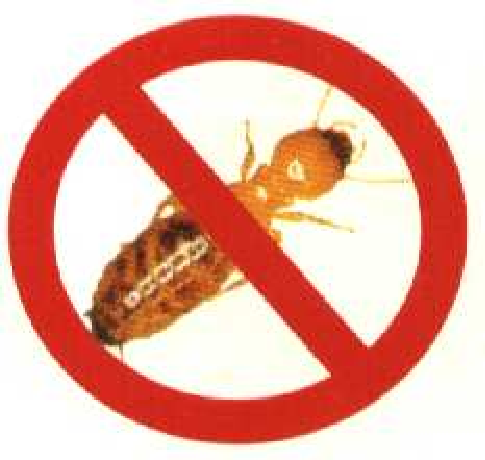
\includegraphics[width=0.5\textwidth]{Cap1/cupim}
\caption{Proibido estacionar cupins. Legenda grande, com o objetivo de demonstrar a indentação na lista de figuras.}
\label{cupim}
\end{figure}

\chapter{Revsião da literatura}
\section{templates}

Exemplo de uma tabela.

\begin{table}[ht]
\caption{Exemplo de uma Tabela}
\label{minhatab}

\center
\begin{tabular}{cccc}
  % after \\: \hline or \cline{col1-col2} \cline{col3-col4} ...
  \hline
	Parâmetro & Unidade & Valor da simulação & Valor experimental   \\
	\hline
  Comprimento, $\alpha$ & $m$ &  $8,23$  & $8,54$ \\
  Altura, $\beta$ & $m$     &  $29,1$ & $28,3$\\
	Velocidade, $v$ & $m/s$  &  $60,2$ & $67,3$\\
	\hline
\end{tabular}
\end{table}

% Exemplo de uma imagem.

% \begin{figure}[ht]
% \centering
% 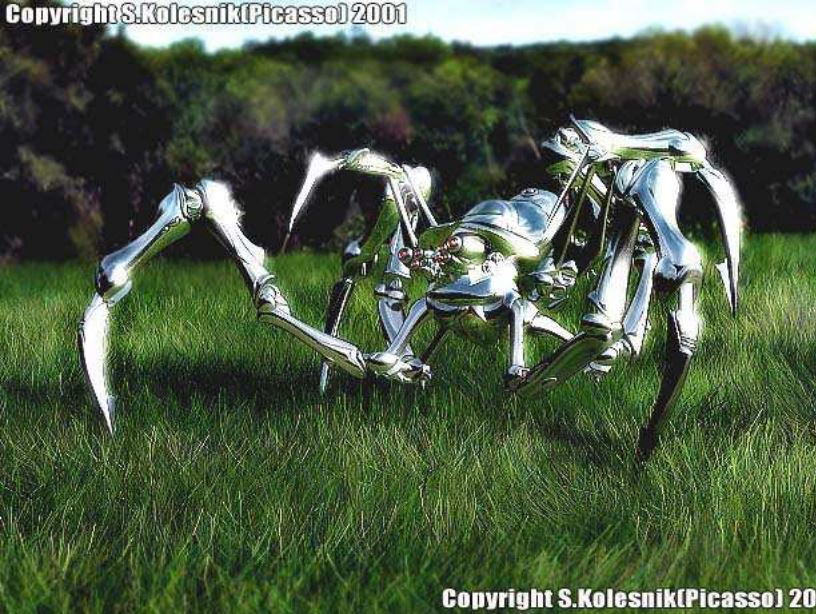
\includegraphics[width=0.75\textwidth]{Cap2/spiderrobot}
% \caption{Cupim cibernético.}\label{fig:cupim}
% \end{figure}


Exemplo de uma equação

\begin{equation} \label{eq:lagr1}
\frac{d}{dt}(\frac{\partial L}{\partial \dot{q}})-\frac{\partial L}{\partial q}=\tau^{T}.
\end{equation}



\chapter{Metodologia}
\section{Materiais e caracterização}
\label{sec:materiais_e_caracterizacao}

Para o desenvolvimento das argamassas geopoliméricas monocomponentes, utilizaram-se os seguintes componentes:

\begin{itemize}
    \item Metacaulim (MK) fornecido pela empresa \textcolor{red}{XXX};
    \item Sílica ativa (SF) fornecida pela empresa \textcolor{red}{XXX};
    \item Carbonato de potássio sólido da empresa \textcolor{red}{XXX};
    \item Hidróxido de cálcio da empresa \textcolor{red}{XXX};
    \item Areia padronizada de quartzo da empresa \textcolor{red}{XXX};
    \item Água destilada.
\end{itemize}

Os aglomerantes utilizados foram a sílica ativa e o metacaulim. Entretanto, a pureza encontrada no mercado do metacaulim não é suficiente para garantir precisão na caracterização das amostras cimentícias.
Portanto, ele foi produzido a partir do caulim comercial, conforme detalhado na Seção \ref{sec:producao_do_metacaulim}.
Já as fontes alcalinas são encontradas no mercado com alta pureza, portanto foi utilizada a composição físico-química fornecida pelo fabricante.

A composição química dos materiais empregados na formulação das argamassas é apresentada na Tabela \ref{tab:composicao_quimica_reagentes}.

\begin{table}[H]
    \caption{Propriedades químicas dos reagentes sólidos.}
    \label{tab:composicao_quimica_reagentes}
    \center
    \begin{tabular}{ccc}
    % after \\: \hline or \cline{col1-col2} \cline{col3-col4} ...
        \hline
        Material & Composição química & Especificação (\%)\\
        \hline
        Sílica ativa & $SiO_2$ &  \textcolor{red}{XX,X} \\
            & $ Al_2O_3$ & \textcolor{red}{XX,X} \\
            & $MgO$ & \textcolor{red}{XX,X} \\
            & $CaO$ & \textcolor{red}{XX,X} \\
            & $Fe_2O_3$ & \textcolor{red}{XX,X} \\
        Carbonato de potássio & $K_2CO_3$ & \textcolor{red}{XX,X} \\
        Hidróxido de cálcio & $Ca(OH)_2$ & \textcolor{red}{XX,X} \\
        \hline
    \end{tabular}
\end{table}

Além disso, a areia de quartzo utilizada segue os padrões estabelecidos pelo Instituto de Pesquisas Tecnológicas (IPT), representados nas Tabelas \ref{tab:areia_quartzo_propriedades} e \ref{tab:areia_quartzo_granulometria}.

\begin{table}[H]
    \caption{Resultados de requisitos fisicos e químicos da areia de quartzo padronizada.}
    \label{tab:areia_quartzo_propriedades}
    \center
    \begin{tabular}{p{0.25\textwidth} p{0.25\textwidth} p{0.25\textwidth}}
        \hline
        Propriedade & Resultado & Requisito ABNT NBR 7214:2015 \\
        \hline
        Teor de sílica (ABNT NBR 14656:2001) & 96,5\% & $\geq$ 95\%, em massa \\
        Umidade (ABNT NBR 7214:2015) & 0,0\% & $\leq$ 0,2\%, em massa \\
        Matéria orgânica (ABNT NBR 17053:2022) & Mais clara ou igual à cor da solução padrão & Cor da solução padrão de ácido tânico a 2\% \\
        \hline
    \end{tabular}
\end{table}

\begin{table}[H]
    \caption{Composição granulométrica das frações da areia de quartzo padronizada.}
    \label{tab:areia_quartzo_granulometria}
    \centering
    \begin{tabular}{p{0.10\textwidth} p{0.30\textwidth} p{0.15\textwidth} p{0.20\textwidth}}
        \hline
        \multirow{2}{=}{Fração} & \multirow{2}{=}{Intervalo entre peneiras} & \multicolumn{2}{c}{Porcentagem em massa (\%)} \\ \cline{3-4}       
        & & Resultado & Requisito ABNT NBR 7214:2015 \\
        \hline
        16 & (2,4 mm e 2,0 mm) & 0 & $\leq$ 10 \\
        16 & (2,0 mm e 1,2 mm) & 97 & $\geq$ 90 \\
        30 & (1,2 mm e 0,6 mm) & 99 & $\geq$ 95 \\
        50 & (0,6 mm e 0,3 mm) & 96 & $\geq$ 95 \\
        100 & (0,3 mm e 0,15 mm) & 95 & $\geq$ 95 \\
        \hline
    \end{tabular}
\end{table}

\section{Produção do metacaulim}
\label{sec:producao_do_metacaulim}

O metacaulim foi obtido a partir da calcinação do caulim a $700\ ^\circ C$ por 1 hora, em um forno elétrico da marca \textcolor{red}{XXX}.
O tempo de calcinação e temperatura ótimos foram determinados a partir de ensaios prévios, onde foi avaliado o rendimento da calcinação.
Para garantir a homogeneidade do material, foram utilizadas duas formas rasas com altura máxima de \textcolor{red}{XX} mm.
A transformação da caulinita cristalina em metacaulinita amorfa é representada pela Equação \ref{eq:calcinacao_caulim}.

\begin{equation}
    \label{eq:calcinacao_caulim}
        Al_2.2Si_2O_2.2H_2O \xrightarrow{\Delta} Al_2O_3.2SiO_2 + 2 H_2O
\end{equation}

\section{Caracterização físico-química dos precursores sólidos}
\label{sec:caracterizacao_fisico_quimica_dos_precursores_solidos}

A caracterização físico-química dos precursores sólidos foi realizada nos laboratórios do Instituto Tecnológico de Aeronáutica (ITA), localizado em São José dos Campos-SP.

A espectroscopia de energia dispersiva de raios-X (EDS) permitiu determinar a proporção dos elementos químicos, realizada juntamente com a microscopia eletrônica de varredura (SEM) para avaliação da morfologia dos precursores sólidos.

Além disso, a difração de raios-X (XRD) foi utilizada para determinar a fase cristalina do metacaulim e da sílica ativa.

% A determinação da composição química dos materiais precursores (metacaulim, escória de alto forno e sílica ativa) foi realizada no Centro de Desenvolvimento Técnico Nuclear (CDTN), localizado na Universidade Federal de Minas Gerais (UFMG), por meio do espectrômetro de energia dispersiva de raios X (EDS), modelo EDX-720 da Shimadzu, utilizando-se um método quantitativo. A composição mineralógica desses materiais foi obtida por meio de difração de raios X, empregando-se um difratômetro da marca Shimadzu, modelo XRD-7000, com radiação de cobre (Cu-Kα, λ = 1,5418 Å), operando a 40 kV e 30 mA. Para a determinação das fases cristalinas, foram realizadas varreduras com velocidade angular de 0,02° por segundo, dentro de um intervalo de medida entre os ângulos de Bragg (2θ) de 5° a 80°.

A fim de verificar a remoção dos grupos hidroxilas ($OH^-$) e a presença das ligações $Al-Si-O$, foi realizada a espectroscopia de infravermelho (FTIR) em um espectrômetro da marca \textcolor{red}{XXX}.

Por fim, a distribuição do tamanho de partícula dos sólidos empregados foi realizada através do ensaio de granulometria a laser. Partículas menores e mais irregulares tendem a apresentar maior área superficial específica e, portanto, maior reatividade em contato com a fonte alcalina, o que pode influenciar diretamente no desempenho mecânico e nas propriedades reológicas das argamassas geopoliméricas.

% As distribuições granulométricas do metacaulim (MC), escória de alto forno (EAF) e sílica ativa (SA) foram determinadas por difração a LASER, utilizando-se um equipamento CILAS1090. As amostras foram dispersas em água destilada, e as condições de ensaio adotadas incluíram agitação a 1500 rpm, tempo de ultrassom de 2,5 minutos, obscuração entre 10 e 20%, e tempo total de dispersão de 5 minutos.

\section{Produção das argamassas e pastas geopoliméricas}
\label{sec:producao_das_argamassas_e_pastas_geopolimericas}

\subsection{Formulação das misturas}
\label{subsec:formulacao_das_misturas}

O desenvolvimento das argamassas geopoliméricas monocomponentes seguiu um planejamento experimental sistemático, visando avaliar o efeito das diferentes composições nas propriedades físico-químicas e mecânicas.

As variáveis consideradas no estudo foram:

\begin{itemize}
    \item Proporção entre os precursores sólidos (metacaulim e sílica ativa);
    \item Teor de ativadores alcalinos ($K_2CO_3$ e $Ca(OH)_2$);
    \item Relação água/sólidos (a/s);
    \item Relação areia/material cimentício (ar/c).
\end{itemize}

A variável de estudo deste experimento é a relação $Si/Al$, que será variada de 1,0 até 5,0, sendo a relação $Si/Al$ calculada com base na proporção de metacaulim e sílica ativa.

Inicialmente, a proporção de água/sólidos foi determinada de maneira análoga a \textcolor{red}{ref xxxx}, visando garantir a trabalhabilidade adequada das pastas.

Além disso, devido ao balanço estequiométrico, a relação $Al/K$ será constante e igual a 1, conforme a fórmula empírica \ref{eq:relacao_al_k} \cite{joseph1991geopolymers}, onde $M$ é um cátion de sódio ou potássio.

\begin{equation}
    \label{eq:relacao_al_k}
    M_n \left\{ \left(SiO_2 \right)_z AlO_2 \right\}_n \cdot wH_2O
\end{equation}

Ademais, a relação $K/Ca$ será constante e igual a 2, respeitando a reação de precipitação do carbonato de potássio com o hidróxido de cálcio, conforme a Equação \ref{eq:reacao_k_ca}.

\begin{equation}
    \label{eq:reacao_k_ca}
    K_2CO_3 + Ca(OH)_2 \rightarrow  2KOH_{(aq)} + CaCO_{3(s)} \downarrow
\end{equation}

Tendo as proporções da pasta bem definidas, a produção das argamassas manteve a proporção de 1:3 entre o aglomerante e a areia, conforme a literatura \textcolor{red}{ref XXXX}.

% For the chemical designation of geopolymers based on silico-aluminates, poly(sialate) was suggested. Sialateis an abreviation for silicon-oxo-aluminate. The sialate network consists of SiO4 and AlO4 tetrahedra linkedalternately by sharing all the oxygens. Positive ions (Na+, K+, Li+, Ca++, Ba++, NH4+, H3O+) must bepresent in the framework cavities to balance the negative charge of Al3++ in IV-fold coordination.Poly(sialates) have this empirical formula

A Tabela \ref{tab:composicoes_argamassas} apresenta as diferentes formulações produzidas, com as respectivas proporções em massa dos componentes.

\begin{table}[H]
    \caption{Composições das argamassas geopoliméricas produzidas.}
    \label{tab:composicoes_argamassas}
    \center
    \begin{tabular}{cccccccc}
    \hline
    Amostra & \multicolumn{2}{c}{Precursores (\%)} & \multicolumn{2}{c}{Ativadores (\%)} & \multirow{2}{*}{a/s} & \multirow{2}{*}{ar/c} & \multirow{2}{*}{Si/Al} \\
    \cline{2-5}
     & MK & SF & $K_2CO_3$ & $Ca(OH)_2$ & & \\
    \hline
     AGP1 & \textcolor{red}{XX} & \textcolor{red}{XX} & \textcolor{red}{X,X} & \textcolor{red}{X,X} & \textcolor{red}{X,XX} & \textcolor{red}{X,X} & \textcolor{red}{1,0} \\
    AGP2 & \textcolor{red}{XX} & \textcolor{red}{XX} & \textcolor{red}{X,X} & \textcolor{red}{X,X} & \textcolor{red}{X,XX} & \textcolor{red}{X,X} & \textcolor{red}{2,0} \\
    AGP3 & \textcolor{red}{XX} & \textcolor{red}{XX} & \textcolor{red}{X,X} & \textcolor{red}{X,X} & \textcolor{red}{X,XX} & \textcolor{red}{X,X} & \textcolor{red}{3,0} \\
    AGP4 & \textcolor{red}{XX} & \textcolor{red}{XX} & \textcolor{red}{X,X} & \textcolor{red}{X,X} & \textcolor{red}{X,XX} & \textcolor{red}{X,X} & \textcolor{red}{4,0} \\
    AGP5 & \textcolor{red}{XX} & \textcolor{red}{XX} & \textcolor{red}{X,X} & \textcolor{red}{X,X} & \textcolor{red}{X,XX} & \textcolor{red}{X,X} & \textcolor{red}{5,0} \\
    \hline
    \end{tabular}
\end{table}

\subsection{Procedimento de mistura}
\label{subsec:procedimento_de_mistura}

A produção das misturas seguiu os procedimentos normatizados.
Para a produção das argamassas e ensaio de compressão, seguiram-se os procedimentos da norma brasileira \cite{ABNT_NBR_7215_2019}, já para a produção das pastas, optou-se pela norma americana \cite{ASTM_C305_2006}, uma vez que a norma brasileira não especifica o procedimento de mistura para pastas cimentícias sem agregado miúdo.
Ambos os procedimentos foram adaptados para o preparo de amostras de volume reduzido.

\subsection{Moldagem e cura dos corpos de prova}
\label{subsec:moldagem_e_cura_dos_corpos_de_prova}

Para o ensaio de compressão, os corpos de prova foram preparados em moldes prismáticos de dimensões \textcolor{red}{XX} × \textcolor{red}{XX} × \textcolor{red}{XX} mm, previamente lubrificados com desmoldante à base de óleo.

Para cada composição, foram moldados 9 corpos de prova, destinados aos ensaios nas idades de 1, 3 e 7 dias (3 corpos de prova para cada idade). Não foi necessário realizar os testes aos 28 dias, pois a cura térmica dos aglomerantes empregados apresenta alto ganho de resistência inicial, conforme demonstrado na literatura \textcolor{red}{ref XXX}.

Optou-se por realizar a cura térmica em uma estufa mantida a (60 ± 2)°C e umidade relativa mínima de 95\% por 24 horas, conforme recomendado na norma \cite{ABNT_NBR_9479_2006}, para garantir a ativação dos aglomerantes e acelerar o processo de cura.
Vale ressaltar que o desmolde foi realizado 24 horas após o início do processo de cura.

A desmoldagem foi realizada após 24 horas da moldagem, e os corpos de prova foram imediatamente transferidos para as condições de cura correspondentes até a idade de ensaio.

Para as análises microestruturais, pequenas amostras foram separadas, tendo a hidratação interrompida por imersão em álcool etílico e filtragem a vácuo, seguida de secagem em estufa a 40°C por 24 horas. Tais amostras foram armazenadas em recipientes herméticos para evitar uma nova hidratação.

\section{Caracterização das misturas geopoliméricas}
\label{sec:caracterizacao_das_misturas_geopolimericas}

\subsection{Ensaios no estado endurecido}
\label{subsec:ensaios_no_estado_endurecido}

\subsubsection{Resistência à compressão}
\label{subsubsec:resistencia_a_compressao}

Para o ensaio de resistência à compressão, os corpos de prova foram inseridos em uma prensa hidráulica da marca \textcolor{red}{XXX}, modelo \textcolor{red}{XXX}, aplicando-se carga com velocidade de \textcolor{red}{XXX} N/s até a ruptura. A resistência foi calculada pela equação:

\begin{equation}
    \label{eq:resistencia_compressao}
    R_c = \frac{F_c}{A_t}
\end{equation}

Onde:
\begin{itemize}
    \item $R_c$ é a resistência à compressão, em MPa;
    \item $F_c$ é a carga máxima aplicada, em N;
    \item $A_t$ é a área da seção transversal, em mm\textsuperscript{2}.
\end{itemize}

Para análise estatística, realizou-se o teste de Tukey, permitindo identificar diferenças significativas entre os grupos de amostras, considerando um nível de significância de \textcolor{red}{XXX}\%.

\subsection{Análises microestruturais}
\label{subsec:analises_microestruturais}

\subsubsection{Difração de raios X (XRD)}
\label{subsubsec:difracao_de_raios_x}

As análises de difração de raios X foram realizadas em amostras moídas das pastas, com granulometria inferior a 75 µm, nas idades de 7 e 28 dias. Utilizou-se um difratômetro da marca \textcolor{red}{XXX}, modelo \textcolor{red}{XXX}.
%  com radiação de cobre (Cu-Kα, λ = 1,5418 Å), operando a 40 kV e 30 mA. As varreduras foram realizadas com velocidade angular de 0,02° por segundo, em um intervalo de 5° a 80° (2θ).

\subsubsection{Espectroscopia de infravermelho por transformada de Fourier (FTIR)}
\label{subsubsec:espectroscopia_de_infravermelho}

A espectroscopia de infravermelho foi realizada em amostras moídas das pastas, com granulometria inferior a 45 µm, nas idades de 1, 3 e 7 dias. Utilizou-se um espectrômetro da marca \textcolor{red}{XXX}, modelo \textcolor{red}{XXX}, na faixa de \textcolor{red}{XXX} a \textcolor{red}{XXX} cm$^{-1}$, com resolução de \textcolor{red}{XXX} cm$^{-1}$ e \textcolor{red}{XXX} varreduras. 

\subsubsection{Microscopia eletrônica de varredura (SEM)}
\label{subsubsec:microscopia_eletronica_de_varredura}

A análise microestrutural das pastas foi realizada por microscopia eletrônica de varredura, utilizando um microscópio da marca \textcolor{red}{XXX}, modelo \textcolor{red}{XXX}, acoplado a um espectrômetro de energia dispersiva de raios X (EDS). As amostras foram preparadas a partir de fragmentos cilíndricos das pastas moldadas em um canudo de plástico descartável. 
% As análises foram realizadas com ampliações de 500×, 2000× e 5000×, com tensão de aceleração de 15 kV.



\chapter{Resultados e discussão}
%\section{Conclusão}

Neste trabalho realizou-se o projeto de uma metodologia de controle subótimo redundante da junta passiva de um manipulador com três graus de liberdade instantaneamente. Para este propósito usou-se nas formulações o vetor gradiente de uma função escalar que estima o acoplamento entre a junta passiva e as ativas desse manipulador. Aqui a redundância
foi usada da melhor maneira possível sem focalizar o efeito global. Portanto, este método deve ser denominado de \emph{controle ótimo local por redundância}. A principal vantagem dessa formulação é a computação em tempo real, que é
necessária para o controle do manipulador experimental. Além disso esse método pode ser usado com diferentes tipos de controladores, uma vez que as alterações são feitas nas equações dinâmicas do manipulador.

A consequência direta observada nessa formulação é a redução dos torques na fase de controle da junta passiva, e consequente redução da energia elétrica gasta. Isso ocorre devido ao fato de que ao longo da trajetória do manipulador
o índice de acoplamento de torque tende a ser maximizado, e portanto, menor é o torque necessário nos atuadores para se conseguir o posicionamento da junta passiva do manipulador.

Outros resultados indiretos obtidos são: um movimento mais uniforme e suave do manipulador e um tempo de acomodação menor tanto no posicionamento da junta passiva quanto das ativas, conforme podemos obervar nos gráficos de desempenho dos resultados apresentados. Isso ocorre porque a maximização do acoplamento entre as juntas facilita o controle. Assim
ocorrem menos picos de torque, e como as juntas ativas tem ``menos trabalho'' para posicionar a passiva estas se movem menos na direçao contrária ao movimento daquelas, diminuindo assim as velocidades alcançadas e os tempos de posicionamento.

Uma extensão deste trabalho pode ser a implementação de um \emph{controle ótimo global por redundância} da junta passiva do manipulador. Para isto pode-se fazer o planejamento \emph{off-line} da trajetória das juntas de modo a minimizar a energia consumida. Alguns estudos foram feitos nesse sentido, usando o Princípio Mínimo de Pontryagin, mas sem resultados satisfatórios até o momento.


\chapter{Conclusão}
Lorem ipsum dolor sit amet, consectetur adipiscing elit. Nullam venenatis augue id augue ultrices, et gravida magna vehicula. Cras volutpat suscipit iaculis. Praesent varius ac orci sed ultrices. Vivamus vestibulum molestie lorem. Maecenas id congue tortor. Aliquam erat volutpat. Nullam ornare tortor et nunc sagittis laoreet. Sed at turpis et quam facilisis elementum. Nullam ultrices elit ut accumsan ultricies. Nulla sit amet tellus lacus. Vestibulum ac lectus velit. Donec nunc odio, mattis nec orci sed, porta lobortis lectus.

Proin ultricies elit vitae mi efficitur eleifend. Nulla non lorem consectetur, placerat dui quis, feugiat urna. Quisque sed ligula massa. Donec finibus placerat orci, eget mollis justo rutrum a. Sed luctus feugiat congue. Phasellus libero felis, tempor quis rutrum pretium, porttitor ac nisi. Praesent euismod malesuada enim a rhoncus. Aliquam gravida fringilla aliquam. Proin nunc lorem, convallis fringilla eleifend et, tempus quis orci. Phasellus bibendum, tellus eu elementum posuere, odio lacus maximus eros, nec lobortis lectus nisi a turpis. Vivamus viverra felis et dolor viverra interdum. Nulla convallis nisi eu sapien egestas aliquet sit amet eget risus. Phasellus vel quam vel lacus commodo lacinia.

Donec ultrices ac nisi nec elementum. Aenean pellentesque pellentesque pulvinar. Ut aliquet nulla vitae porttitor hendrerit. Nullam venenatis nisl nec ipsum malesuada ultricies. Curabitur massa erat, auctor in ipsum non, semper ornare nunc. Donec non felis eget diam porta rhoncus. Mauris id lectus sed arcu iaculis dictum et vitae velit. Cras sit amet neque vel sapien interdum fermentum sit amet eu lorem. Fusce urna sem, pretium a facilisis id, aliquet at mi. Etiam elementum eget est et porttitor. Morbi ultricies lorem a arcu mattis, eget egestas ex ultrices. Pellentesque bibendum sed est ac imperdiet.

% REFERENCIAS BIBLIOGRAFICAS
\renewcommand\bibname{\itareferencesnamebabel} %renomear título do capítulo referências
\bibliography{Referencias/referencias}

% Apendices
\appendix
\chapter{Tópicos de Dilema Linear} %opcional
\section{Uma Primeira Seção para o Apêndice}

A matriz de Dilema Linear $M$ e o vetor de torques inerciais $b$,
utilizados na simulação são calculados segundo a formulação 
abaixo:
\begin{equation}
M=\left[ \begin{array}{ccc}
M_{11} & M_{12} & M_{13} \\
M_{21} & M_{22} & M_{23} \\
M_{31} & M_{32} & M_{33}
\end{array} \right]
\end{equation}

\begin{figure}[h]
\centering
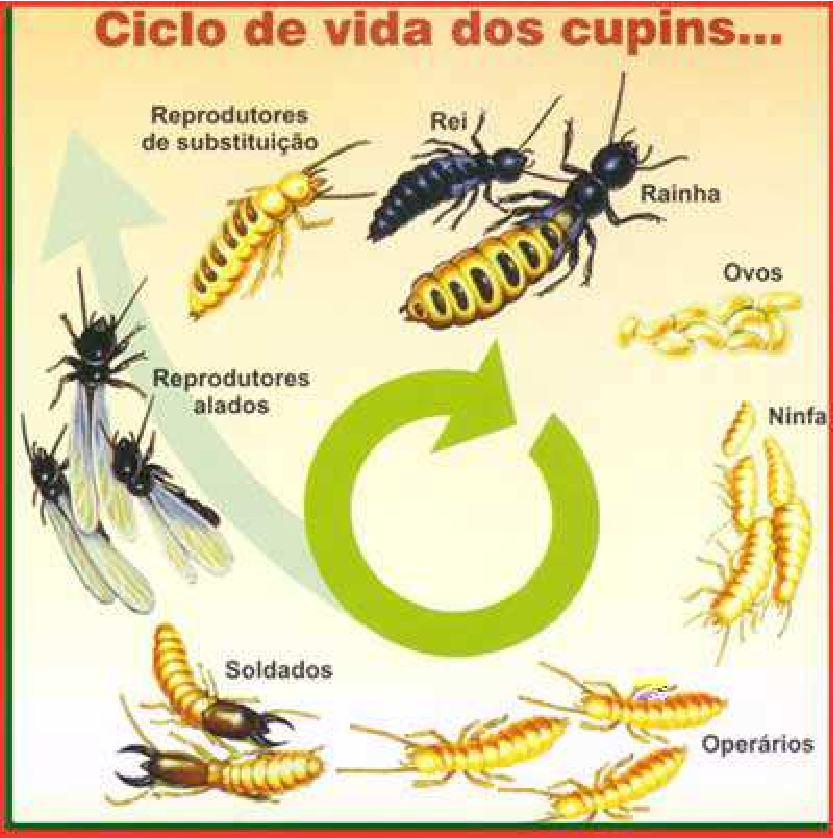
\includegraphics[height=5cm, width=5cm]{ApeA/pragas_ciclo_cupim}
\caption{Uma figura que está no apêndice}\label{FD}
\end{figure}


% Anexos
\annex
\chapter{Exemplo de um Primeiro Anexo} %opcional
% Texto do Primeiro Anexo
\section{Uma Seção do Primeiro Anexo}
% Texto da primeira secao do primeiro anexo
Algum texto na primeira seção do primeiro anexo.



% Glossario
%\itaglossary
%\printglossary

% Folha de Registro do Documento
% Valores dos campos do formulario
\FRDitadata{26 de maio de 2025}
\FRDitadocnro{DCTA/ITA/DM-018/2025} %(o número de registro você solicita a biblioteca)
\FRDitaorgaointerno{Instituto Tecnológico de Aeronáutica -- ITA}
%Exemplo no caso de pós-graduação: Instituto Tecnol{\'o}gico de Aeron{\'a}utica -- ITA
\FRDitapalavrasautor{Cupim; Cimento; Estruturas}
\FRDitapalavrasresult{Cupim; Dilema; Construção}
%Exemplo no caso de graduação (TG):
%\FRDitapalavraapresentacao{Trabalho de Graduação, ITA, São José dos Campos, 2015. \NumPenultimaPagina\ páginas.}
%Exemplo no caso de pós-graduação (msc, dsc):
\FRDitapalavraapresentacao{ITA, São José dos Campos. Curso de Graduação. Programa de Graduação em Engenharia Civil-Aeronáutica. Departamento de Estruturas e Edificações. Orientador: Prof.~Dr. João Cláudio Bassan de Moraes . Coorientadora: Pamela Rodrigues Passos Severino. Defesa em 26/05/2025. Publicada em 26/05/2025.}
\FRDitaresumo{Na busca por alternativas mais sustentáveis ao cimento Portland, os cimentos ativados
alcalinamente têm sido amplamente estudados. No entanto, a maioria dos processos
de mistura ocorre em duas etapas, o que impacta a viabilidade e a eficiência
construtiva. Um avanço importante nessa área é o desenvolvimento de sistemas
monocomponentes, que simplificam a produção e tornam a tecnologia mais acessível
e prática. Ainda assim, os estudos atuais se concentram em precursores ricos em
cálcio, enquanto o uso de fontes alcalinas tradicionais apresenta desafios relacionados
à segurança e ao custo. Este trabalho propõe o desenvolvimento de um cimento
ativado alcalinamente monocomponente utilizando precursores sólidos de baixo teor
de cálcio, como sílica ativa e metacaulim, e fontes alcalinas mais seguras e acessíveis,
como carbonato de potássio e hidróxido de cálcio, garantindo resistência mecânica
adequada e maior viabilidade para aplicação na construção civil.}
%  Primeiro Parametro: Nacional ou Internacional -- N/I
%  Segundo parametro: Ostensivo, Reservado, Confidencial ou Secreto -- O/R/C/S
\FRDitaOpcoes{N}{O}
% Cria o formulario
\itaFRD

\end{document}
% Fim do Documento. O massacre acabou!!! :-)
